\graphicspath{{chapters/03/images/}}
\chapter{Extracellular matrix - ECM}

\section{Introduction}

	\subsection{ECM functional role}
	The extracellular matrix provides a starting point for scaffold biodesign in tissue engineering.
	It is a dynamic environment produced and regulated by cells which performs different functions:

	\begin{multicols}{2}
		\begin{itemize}
			\item Aids in cell locomotion through transmembrane receptors and ligands in the ECM.
				This adhesion ligands are patterned in order to direct cell locomotion in a specific direction.
			\item Transmits and distributes mechanical loads: the ECM assumes a specific structure in order to transmit mechanical stresses to the cell in a tissue-specific manner.
			\item Prevents premature mechanical failure.
			\item Partitions cells and tissues into functional units.
			\item Acts as a scaffold defining tissue and organ architecture.
			\item Acts as a storage and dissipative device for elastic energy.
			\item Acts as substrate for cell adhesion, growth, and differentiation.
				Adhesion is the activation step that allows for cell growth and differentiation, and because of this it fundamental for the activation of regenerating cells.
		\end{itemize}
	\end{multicols}

	The ECM is a controlled complex network composed of proteins, glycoproteins and proteoglycans (PGs), which assemble in a tissue-specific manner to provide tissue specific biophysical and biochemical properties.

		\subsubsection{ECM-cell interaction}
		The interaction of the ECM with the cells is necessary as to avoid cells entering into a pathogenic state.
		Cell's nuclei and the ECM interact through integrins.
		This integrins convert external signals into a context-specific gene expression profile.
		The ability of cells to sense the chemical, mechanical and topographical features of the ECM enables them to integrate complex, multiparametric information into a coherent response to the surrounding microenvironment.
		Consequently, dysregulation or mutation of ECM components results in a broad range of pathological conditions.
		Because of this the ECM can be considered as a composite material where cells sense the environment.
		ECM polymers or networks are instructive: they provide structural and mechanical integrity to tissues.
		A tissue engineering scaffold should activate this integrins and ligands as to activate the gene expression profile necessary for regeneration.
		The focus should be on activating the correct pathway as to have the desired therapeutic effect and not a damage one.

		\subsubsection{Regulating cells' fate}
		The ECM controls whether a cell should undergo apoptosis or necrosis.
		Apoptosis is a programmed cell death, in which cells are encapsulated by vesicles and removed.
		Necrosis instead happens when the cellular membrane is damaged, causing the rupture of the cell and inflammation.
		During necrosis the activity of macrophages is increased, producing also inflammation for neighbouring cells.
		It has been suggested to induce tumour cell death through apoptosis to avoid upregulating inflammation.

	\subsection{Components of the ECM}
	The ECM is composed of different molecules:

	\begin{multicols}{2}
		\begin{itemize}
			\item Physical signals: fibronectin, vitronectin, collagen, laminin, fibrillin, glycosamminoglycans (GAGs), PGs.
			\item Soluble signals: growth factors (GF), cytokines, chemokines, used for communicating with distant cells.
			\item Structure: fiber-based and function dependent composites.
			\item Water: tune mechanical properties to better support compressive stress.
				Highly present in articular cartilage, its content is controlled by GAGs and PGs.
			\item Mechano-transduction: translating mechanical stimuli.
		\end{itemize}
	\end{multicols}

		\subsubsection{Collagen fibers}
		The ECM is composed mostly of collagen fibres, which can be organized into:

		\begin{multicols}{2}
			\begin{itemize}
				\item Fibrils, very elastic structures.
				\item Fibres: more thicker and stiff than fibrils.
				\item Bundles: composition of bundled fibres.
			\end{itemize}
		\end{multicols}

		To better tune the mechanical properties without changing the ECM's chemistry the orientation of the fibres will change, depending on the external mechanical stimuli.
		Change the organization of the fibres cause modifications in water content and rigidity, causing a completely different signal to be sent to the cells communicating with the ECM.

		\subsubsection{Signals}
		Signals are fundamental for cell adhesion and must be considered when designing a scaffold together with ligands and collagen.
		To reduce scaffold complexity by decreasing the number of molecule necessary in a scaffold multifunctional polymers are being developed.
		The cross-talk between cells and the ECM allows for the control of many processes like:

		\begin{multicols}{3}
			\begin{itemize}
				\item Pattern formation.
				\item Morphogenesis.
				\item Cell fate.
				\item Daily cellular processes.
				\item Wound healing.
				\item Tissue homeostasis.
			\end{itemize}
		\end{multicols}

		\subsubsection{Stem cells}
		Stem cells are uniquely capable of reproducing themselves through self-renewing and of differentiating into the different cell types necessary to perform a specialized function.
		They are fundamental in embryogenesis and a control between self-renewal and differentiation is fundamental in the healing process and homeostasis.
		Deregulating this process can cause tumorigenesis, degeneration or a pathogenic state.
		Because of this they are very sensible to the ECM and to the environment.

\section{The matrixome: chemistry of the ECM}

\begin{figure}[ht]
	\centering
	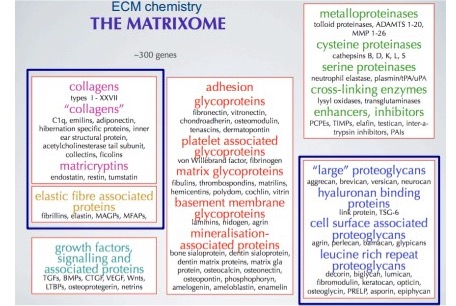
\includegraphics[width=0.8\textwidth]{matrixome}
	\caption{ECM content}
	\label{fig:matrixome}
\end{figure}

Different properties of the ECM are controlled by different molecules, depicted in figure \ref{fig:matrixome}, present in it:

\begin{multicols}{2}
	\begin{itemize}
		\item Stiffness: collagens.
		\item Elasticity: elastic fibres.
		\item Cell-cell communications: signalling molecules like growth factors.
		\item Cell adhesion and mobility direction: adhesion molecules.
		\item Dynamic response: proteinases, which can be used to degrade the scaffold once it is no more needed.
		\item Water content: GAGs and PGs.
	\end{itemize}
\end{multicols}

	\subsection{ECM - cell interaction}
	The cellular membrane is rich in proteins able to sense the external environment and transfer the information to the nucleus, activating a specific gene expression.
	When designing a scaffold, one must provide it the ability to interact with cells with an appropriate mechanism as not to deregulate cellular and tissue mechanisms.

	\begin{figure}[ht]
	\centering
	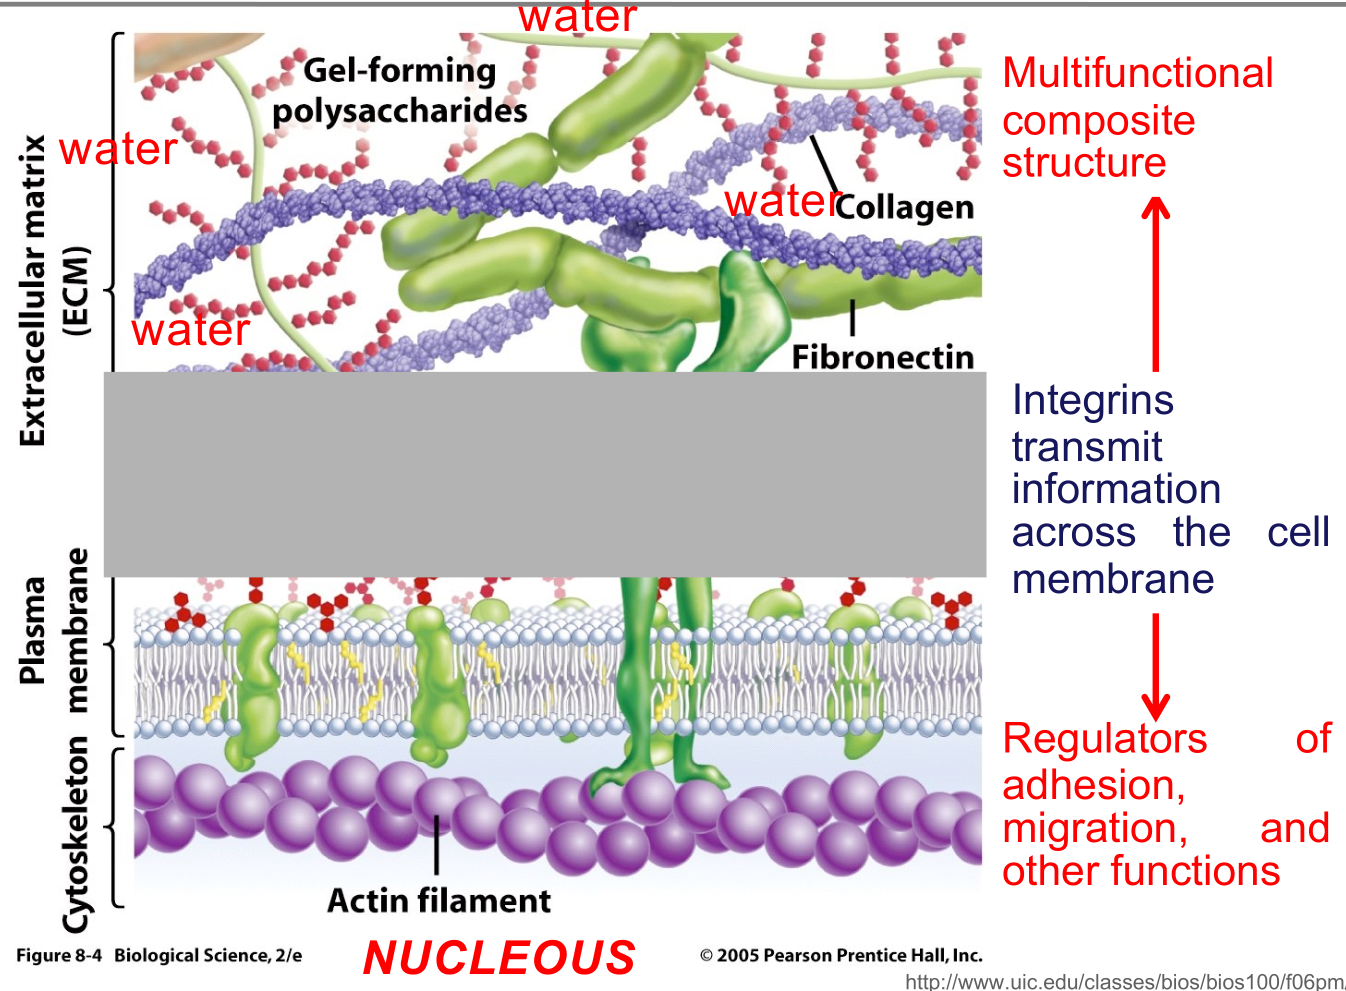
\includegraphics[width=0.6\textwidth]{structure}
	\caption{\label{fig:structure}}
	\end{figure}

	\noindent
	The ECM is a mosaic structure, a guide for cell functions.
	Should the scaffold replicate the ECM? Partially, yes, but especially the functions!
	Large molecules are difficult to manage, maybe using a smaller molecule (nectin instead of fibronectin) is easier.
	Fibronectin is needed to reproduce the complete ECM, but nectin is sufficient to promote cell growth.


	\subsection{Matricellular proteins}
	Matricellular proteins are extracellular modulators of cell function expressed at high level during development and in response to injury.
	They are modulators of cell matrix interactions and bind to many cell surface receptors and to the ECM GFs.
	They are cytokines and proteases.
	Their role is to induce de-adhesion in contrast to the adhesivity of most matrix proteins allowing for cell migration.
	Other functions are:

	\begin{multicols}{2}
		\begin{itemize}
			\item Cell adhesion, migration, chemotaxis.
			\item Matrix assembly and collagen fibrillogenesis.
			\item Regulation proliferation/apoptosis.
			\item Binding/activation GFs and cytokines.
			\item Angiogenesis and tumour growth.
		\end{itemize}
	\end{multicols}

	For example, TSP1 and 2, Tenascon-C and SPARC support a state of intermediate adhesion, with disruption of focal adhesion and the reorganization of actin stress fibres.

	\subsection{Collagen}
	Collagen is one of the most important proteins for the ECM, as it provides structural properties.
	The production of collagen starts in the cytoplasm of cells, while final assembly is performed into the ECM.
	In the ECM collagen assembles into fibrils, then fibres and bundles when needed.
	Collagen is a family of proteins with at least 23 different types.
	Depending on the tissue, there is a prevalence of one type on others.
	In the cartilage for example type II collagen is the most represented, while in tendons it is type III collagen, which is really similar to jellyfish collagen, currently commercialized.

		\subsubsection{Different collagen structures}
		The collagen can assemble in different structure, granting different mechanical properties to the ECM.
		For example:

		\begin{multicols}{2}
			\begin{itemize}
				\item Connective tissue: less density, soft network, more water, fiber and fibrils.
				\item Meniscus: parallel fibers, more density, packed fibers, because of different functions, bundle (more stress).
				\item Myocardium: mechanical stresses, it should support the growth in one direction.
			\end{itemize}
		\end{multicols}

		\subsubsection{Cell-collagen interaction}
		Cells can migrate in a collagen low porosity material through a specific enzymatic process, which allows the opening of the collagen structure.
		A scaffold should be designed to promote cell migration.

		\subsubsection{Chemical characteristics}
		Collagen is non-homogeneous, bottom-up, multi-functional, dynamic and has a hierarchical structure which is function dependent.
		It is composed by three chains that can form an helix formation.
		Controlling the chemical bridges between the chains the elasticity of collagen can be changed.

		\subsubsection{Dynamic nature of the ECM}
		The ECM is degraded by cell-secreted proteases and releasing bioactive components that remodel the collagen structure.
		Natural ECMs modulate tissue dynamics through their ability to locally bind, store and release soluble bioactive ECM effectors such as GFs.

	\subsection{Fibronectin}
	Fibronectin is a large matrix glycoprotein present in most body tissues' fluids.
	Functionally, it is the classic example of an adhesive glycoprotein, binding and interconnecting extracellular matrix components with each other and to the surface of the cells.
	It is one of the most important molecules through which cells interact with the surrounding environment.
	The binding of fibronectin to the cell surface’s integrin receptors plays a critical role in cell migration during the development and postnatally.


		\subsubsection{Chemical characteristics}
	Fibronectin is a dimer composed of two identical chains connected by a disulphide bond.
	Different sections of fibronectin can be recognized:

	\begin{multicols}{2}
		\begin{itemize}
			\item One can interact with fibrin and heparin.
			\item One can interact with gelatine and collagen.
			\item One can interact with the cell receptors through the arg-gly-asp ac. sequence.
			\item One can interact with the polysaccharide heparin.
			\item One can interact with fibrin.
		\end{itemize}
	\end{multicols}

		\subsubsection{Fibronectin interaction}
		Fibronectin is able to interact and crosslink different molecules as to transmit signals and stimuli in the ECM.
		This allows cells to respond quickly to changes in the environment.
		The RGD-loop in fibronectin is strategically placed to undergo strong conformational changes and constitutes a mechanosensitive switch for recognition by integrin receptors.
		Depending on the mechanical stimulus, fibronectin can assume specific conformations, changing its activity and, in doing so, changing the signal that it sends.
	In ECM we have fibronectins, collagen, gel-forming polysaccharides, water, actin and the cell (figure \ref{fig:structure}).

	\subsection{Proteoglycans and GAGs}
	Proteoglycans are composed of a head core protein and a chain of polysaccharides, which is hydrophilic (figure \ref{fig:pgag}).
	The chain of polysaccharides is composed of glycosamminoglycans or GAGs, long linear polysaccharides consisting of repeating disaccharide units, composed of a uronic sugar and an amino sugar, which is usually sulfated.
	Proteoglycans are responsible for controlling the water content of the tissue.
	They aid the ECM in responding do mechanical stresses.
	Many proteoglycans can be linked together via long hyaluronic acid chains, forming giant complexes.
	Because of their negative charges, glycosaminoglycans and proteoglycans together control the water content of the tissue, determining the degree of ”squishiness” of the matrix.
	They also allow for $H_2O$ reentry after tissue compression.
	In fact, during compression, water gets squeezed out and the negative charges of PGs and GAGs draw the escaped water back in when the compression force is no longer in place.

	\begin{figure}[ht]
		\centering
		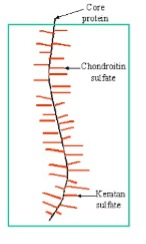
\includegraphics[width=0.3\textwidth]{pgag}
		\caption{\label{fig:pgag}}
	\end{figure}


		\subsubsection{Core protein}
		Glycosaminoglycans are linked to a core proteins in proteoglycans.
		This core protein can be:

		\begin{multicols}{2}
			\begin{itemize}
				\item Hyaluronic acid.
				\item Chondroitin sulfate.
				\item Keratan sulfate.
			\end{itemize}
		\end{multicols}

		The core protein, which is hydrophobic is usually surrounded with hydrophilic molecules.

\section{Modelling nature}
When designing a scaffold the coal is to provide components that will drive tissue regeneration.
The environment in with the scaffold will be implanted is dynamic, with water allowing for most of the interactions.
These interactions regulate a lot of processes, in which there is cell fate, tissue formation and tissue regeneration.
The scaffold needs to allow the cells to work in a natural way, and because of this needs to be modelled based on what is observed in nature.
Living organisms naturally provide a multiplicity of materials, architectures, systems and functions, all resulting from a stringent selection process.
So, a strategy to design a scaffold should include:

\begin{multicols}{2}
	\begin{itemize}
		\item Polymers able to integrate.
		\item Molecular synthesis, done by the cells, at very high level of organisation, allowing molecular recognition, multifunctionality, self-diagnosis and a destruction-recycling process.
		\item Structure dynamics through responsive polymers, allowing for self-assembling, molecule interactions, adaptation and self-healing.
	\end{itemize}
\end{multicols}

The bottom-up approach is more bio-mimetic, as it reflects how nature works: self-assembling blocks, which assemble thanks to the environment to perform a function.
The scaffold design should account for building a context-specific microenvironment.
